\section{Integration in CLAS12}\label{sec:integration}
The FT mechanical design  has been driven by geometrical constraints imposed by the rest of CLAS12, geometrical acceptance optimization and performance optimization, taking into account cooling, material budget, and front-end electronics location.
The FT detects electrons scattered between $2.5^\circ$ an $4.5^\circ$ w.r.t. the beam axis. To provide this acceptance, the FT calorimeter must cover down to $2^\circ$ and up to $5^\circ$ with lead tungstate crystals to have a good containment of E.M. showers at the edges of the polar angular range. Since no massive materials are allowed at angles larger than $5.5^\circ$, crystals, cooling, mechanical supports and tungsten shielding have been optimized in a very compact design. Outside this $5.5^\circ$ we will only have insulating material, which has a very low density, $35\,$kg/m$^3$, and routing for cabling and services in the blind area of the CLAS12 detector, where the torus magnet coils are.

The FT is built by several parts that can be grouped as follow:

\begin{itemize}
\item{the inner tungsten pipe,}
\item{the tungsten cone acting as Moeller electrons shield,}
\item{the tracker,}
\item{the hodoscope,}
\item{the calorimeter,}
\item{the front-end electronics,}
\item{cabling and services.}
\end{itemize}

From the mechanical point of view, the most challenging parts are the integration of the calorimeter, due to the weight and fragility of the crystals and the relative positioning and alignment of the FT components.


\subsection{Constraints from other sub-detectors}

The FT must has be centered on the beam line between the High Threshold Cherenkov Counter (HTCC) and the first layer of Drift Chambers. The HTCC can be retracted in the upstream direction to give access to the FT. In operating position, it extends up to $1730\,$mm downstream w.r.t. the Interaction Point (IP). This plane defines the upstream edge of the allowance for the FT. The first layer of Drift Chambers is installed in front of the toroidal magnet coils, with an inclination of $65^\circ$ w.r.t. the beam axis. The front-end electronics boards of the Drift Chambers define the downstream border of the allowance for the FT. The minimum distance of the Drift Chambers boards from the beam axis is $\sim140\,$mm at $2280\,$mm downstream w.r.t. the IP. Taking into account the outside radius of the FT, including insulation, and the inclination of the Drift Chambers, the FT can not exceed $\sim2150\,$mm w.r.t. the IP.

The FT needs cabling and services routing, for gases and cooling. These services must be connected to the outside of CLAS12. All services are installed in the shadow area of the torus magnet coils, i.e. in six slots extending radially from the beam line to the periphery. Each coil is  $\sim100\,$mm thick, allowing us to host also some front-end electronics, which must be close to the detectors.

The whole FT is attached to the torus magnet cryostat by a support structure with flanges on both ends. This is needed both for mounting sequence constraints and to avoid massive supports in front of the Drift Chambers.  The support structure consists of two concentric stainless-steel pipes connected by adjustment screws to allow for precise alignment and positioning of the detector w.r.t. the beam line and the IP. A third tungsten cylinder of smaller diameter is located inside inside the steel pipes to provide shielding from beam background. 

 The FT is attached to the support structure via the inner tungsten pipe that is part of the calorimeter assembly and is located inside the central holes of the FT detectors. This pipe is designed to hold the entire weight of the FT detectors and of the additional shielding that is mounted upstream of the FT. Tungsten was chosen as material because, even if less resilient, is more rigid than stainless steel reducing the gravitational sagging. The FT-Cal is kept in position w.r.t. the inner tungsten pipe via four radial supports, made of PEEK. PEEK has been chosen because of its low thermal conductivity ($0.25\,$W/m$\cdot$K) and its relatively high tensile strength ($\sim100\,$MPa). In addition, it features high radiation hardness and excellent stability over a broad range of temperatures. Mounting rings in peek and aluminum, respectively, are used to support and align the FT-Hodo and FT-Trk on the inner tungsten pipe.

Upstream of the FT, a tungsten cone is attached to the inner tungsten pipe to provide shielding from Moller electrons produced by the interaction of the beam in the target~\cite{beamline}. Fig.~\ref{fig:integra} shows a section of CLAS12 with the FT in the operating position.

\begin{figure}
\includegraphics[width=1.0\columnwidth]{./fig/IC_integra.eps}
\caption{Forward Tagger installed in CLAS12: on the left, the Cherenkov counter, on the right the toroidal magnet cryostat and one sector of the Drift Chambers. Two boxes for front-end electronics, placed in the cryostat shadow, are shown as well.}
\label{fig:integra}
\end{figure}







\subsection{Cabling and services routing}
All services and cables necessary for the operation of the FT detectors are routed along the torus coils to minimize the interference with the CLAS12 Forward Detector. These include the following items:
\begin{itemize}
\item{FT-Cal:}
\begin{enumerate}
\item{signal cables (332 coaxial cables with diameter of 2 mm),}
\item{HV (4 multiwire cables with diameter of 10 mm) and LV cables (1 multiwire cable with diameter of 12 mm),}
\item{monitoring and slow controls (1 multiwire cable with 14 mm diameter for the readout of the temperature sensors and 6 ethernet cable for the operation of the light monitoring system),}
\item{cooling pipes (2 thermally-insulated pipes with diamater of 35 mm) and gas lines for the nitrogen purge (2 pipes with diameter of 8 mm);}
\end{enumerate}
\item{FT-Hodo:}
\begin{enumerate}
\item{optical fibers (768 1-mm fibers grouped in 48 bundles for a total diameter of 55 mm);}
\end{enumerate}
\item{FT-Trck:}
\begin{enumerate}
\item{optical fibers for the transmission of the digitized signals (6 fibers with diameter of 2 mm),}
\item{slow controls (3 usb cables),}
\item{HV (8 cables) and LV (6 wires with a diameter of 4 mm) cables,}
\item{gas lines (2 pipes with diameter of 12 mm) and cooling lines (3 inlet tubes with diameter of 35 mm).}
\end{enumerate}
\end{itemize}


Cables and pipes are grouped and routed along the direction of the magnet coils using appropriate rails. The rails width and depth has been chosen
to be compatible with  space occupied by  CLAS12 Drift Chambers (both during normal operation  and maintenance) and clearance between the HTCC and the CLAS12 Forward Detector. 

